\section{The Grothendieck Constant}
\label{sec:grothendieck}

We first describe the mathematical problem at a high level. The exposition here is deliberately informal; precise definitions and full proofs appear in the companion paper~\cite{saha2026new}.

\paragraph{A hard optimization problem and its relaxation.}
Consider the following discrete optimization problem: given a matrix $A=(a_{ij})\in\R^{m\times n}$, find sign vectors maximizing the bilinear form
\[
    \OPT(A)
    \;:=\;
    \max_{x\in\{\pm1\}^m,\; y\in\{\pm1\}^n}
    \;\sum_{i,j} a_{ij}\, x_i y_j.
\]
Intuitively, we are looking for the best pair of $\pm1$ labelings of the rows and columns of $A$; this quantity is closely related to the \emph{cut norm} of the matrix, a basic primitive in combinatorial optimization, and the problem is NP-hard in general.
A standard way to make it tractable is to relax each sign to a unit vector and each product to an inner product:
\[
    \SDP(A)
    \;:=\;
    \max_{u_i, v_j \in S^{d-1}}
    \;\sum_{i,j} a_{ij}\, \ip{u_i}{v_j},
\]
where the maximum now runs over unit vectors in any dimension $d$.
This relaxation is a semidefinite program (SDP) and can be solved in polynomial time.
Since every sign is a one-dimensional unit vector, $\OPT(A)\le\SDP(A)$: the relaxation can only overshoot.
The basic question is by how much.

Grothendieck's inequality~\cite{Gro53,LP68} answers this question: the overshoot is bounded by a universal constant.
That is, there exists $K<\infty$, independent of $A$, $m$, $n$, and the dimension $d$, such that
\[
    \OPT(A)
    \;\le\;
    \SDP(A)
    \;\le\;
    K\cdot\OPT(A)
    \qquad
    \text{for every matrix } A.
\]
The \emph{Grothendieck constant} $\KG$ is the smallest such $K$.
In modern language, $\KG$ is exactly the worst-case integrality gap of the canonical SDP relaxation of the bilinear optimization problem above.
\cref{fig:groth-pipeline} illustrates the two optimization problems and the rounding step that connects them.

\begin{figure}[t]
\centering
% Source: paper_artifacts/plots/sdp_workflow_figure.py (parent repo)
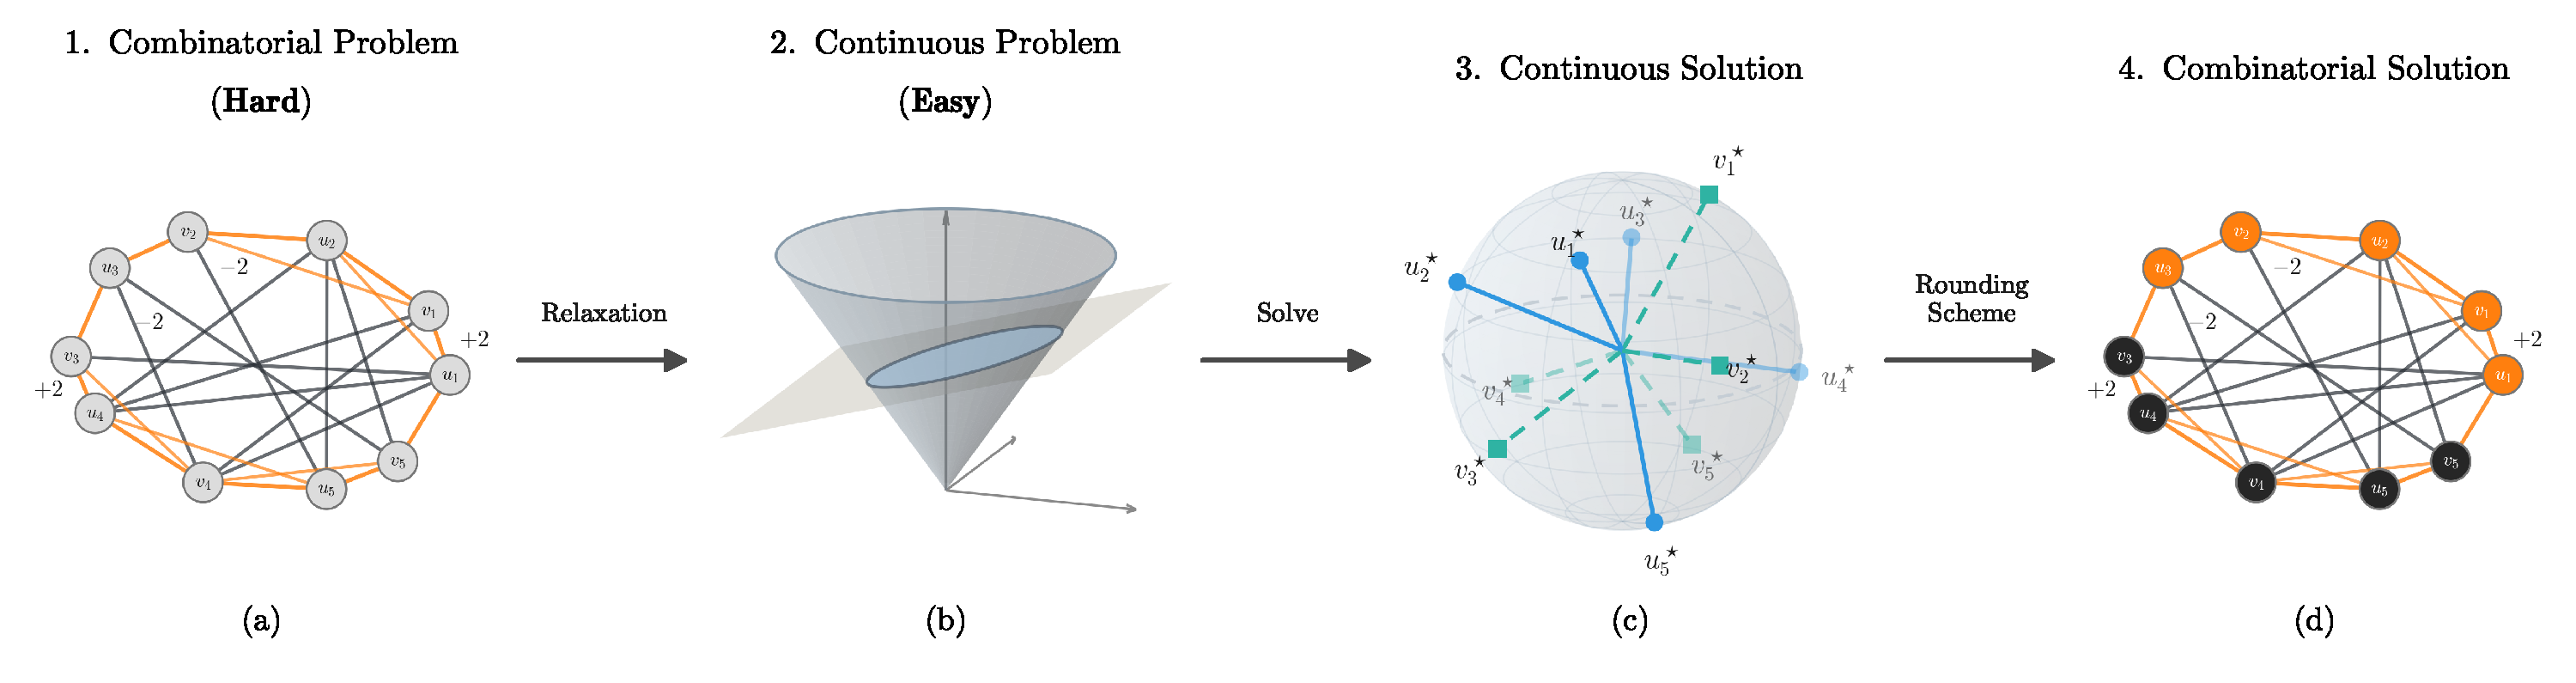
\includegraphics[width=0.9\textwidth]{figures/sdp_workflow}
\caption{\textbf{From a hard combinatorial problem to a rounded solution.}
\emph{(a)} An instance of the bilinear optimization problem, drawn as a weighted graph: every node carries an unknown sign, every edge a weight $a_{ij}$ (an orange $+2$ edge rewards giving its endpoints equal signs; a dark $-2$ edge rewards opposite signs), and the goal is to choose the signs maximizing the total reward.
\emph{(b)} The SDP relaxation replaces signs by unit vectors; its feasible set is a slice of a convex cone, and the relaxed problem is solvable in polynomial time.
\emph{(c)} The optimal vectors $u_i^\star, v_j^\star$ spread out over a unit sphere in ways that signs cannot.
\emph{(d)} A rounding scheme converts the vectors back into signs (orange $=+1$, dark $=-1$); in this instance the rounded signs satisfy every $-2$ edge.
The Grothendieck constant $\KG$ is the worst-case ratio between the relaxed and the combinatorial optimum.}
\label{fig:groth-pipeline}
\end{figure}

Grothendieck's inequality is a foundational result well beyond this algorithmic reading: it originated in functional analysis, where it is central to the geometry of Banach spaces and harmonic analysis~\cite{pisier2011grothendieckstheorempastpresent,KN11}, it underlies constant-factor approximation algorithms for cut norms~\cite{AN06}, and it governs the maximal advantage of quantum over classical correlations in Bell-type experiments~\cite{Tsi85,CHTW04}.
Despite this breadth of connections, and more than seventy years of study, the exact value of $\KG$ remains unknown.

\paragraph{Rounding schemes as partitions.}
Every upper bound on $\KG$ is, at heart, an algorithm: a \emph{rounding scheme} that converts the unit vectors of an SDP solution back into signs while provably retaining a $1/K$ fraction of the objective.
The schemes relevant to this paper have a simple geometric description.
A \emph{Krivine scheme} is a pair of partitions of $\R^k$ into a $+1$ region and a $-1$ region, encoded by odd sign functions $f,g:\R^k\to\{\pm1\}$ (see \cref{fig:partitions}).
To round, the algorithm maps each SDP vector to a random Gaussian point in $\R^k$, arranged so that the points of $u_i$ and $v_j$ are correlated according to the inner product $\ip{u_i}{v_j}$, and then labels each vector by the region its point lands in: $x_i = f(X_i)$ and $y_j = g(Y_j)$.
The simplest instance takes both partitions to be the same half-space, $f(z)=g(z)=\sgn(z_2)$.
This is called the random hyperplane rounding: label each vector by the side of a random hyperplane it falls on.

\begin{figure}[t]
\centering
% Source: figures/make_partition_schemes.py
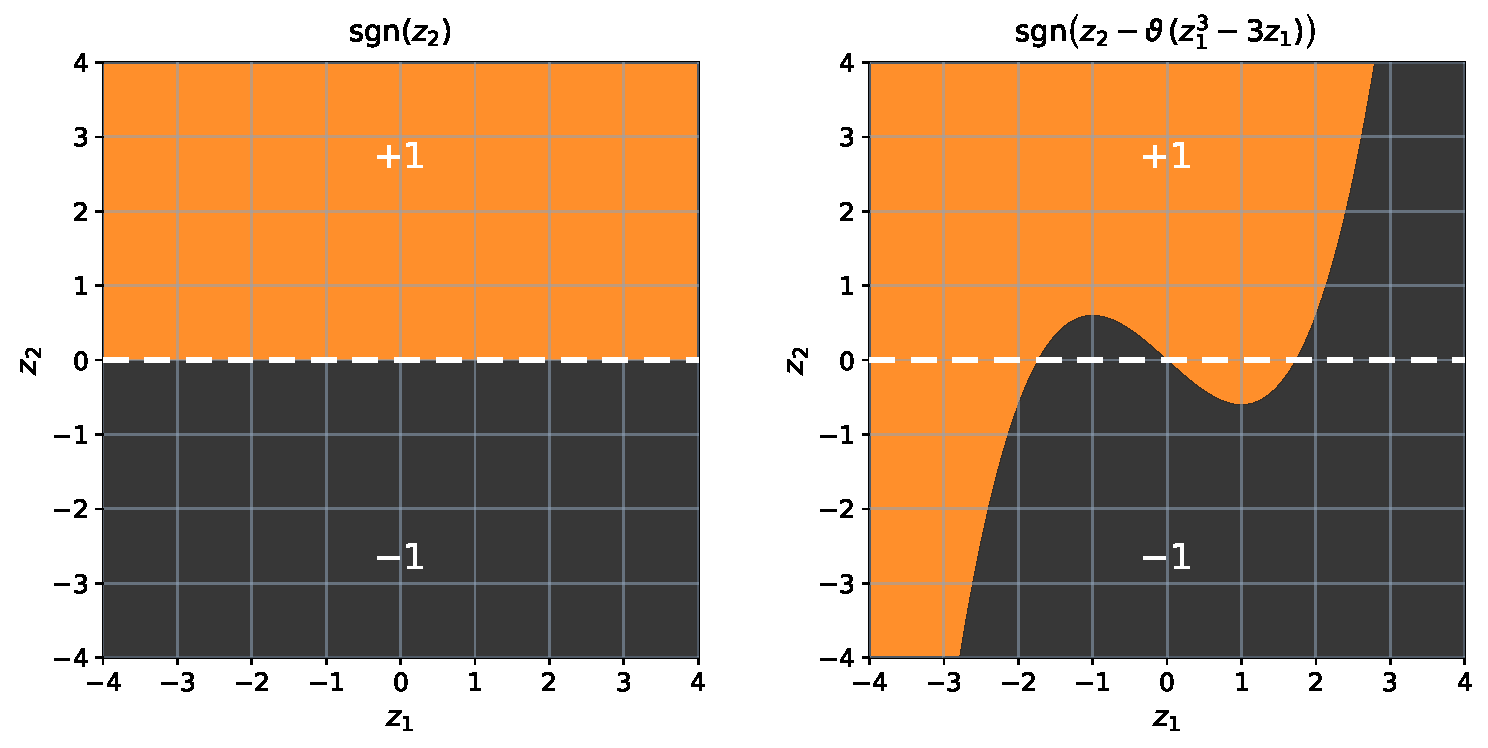
\includegraphics[width=0.85\textwidth]{figures/partition_schemes}
\caption{\textbf{Krivine schemes are partitions of space.}
A scheme labels the points of $\R^k$ with $\pm1$ (orange is $+1$, dark is $-1$; shown here for $k=2$), and each SDP vector is rounded to the label of a correlated random Gaussian point.
\emph{Left:} the half-space partition underlying hyperplane rounding and Krivine's classical bound.
\emph{Right:} a partition with a cubic boundary, of the kind used by the cubic--quintic scheme of the companion paper; the dashed line marks the half-space boundary for comparison.
The extra freedom in the shape of the boundary, combined with the enriched correlation structure of limiting schemes, is what suppresses the nonlinearity of the correlation function $H$.}
\label{fig:partitions}
\end{figure}

\paragraph{The normalized correlation function.}
The quality of a Krivine scheme is governed by a single analytic object.
Let $X,Y$ be standard Gaussian points in $\R^k$ whose coordinates are pairwise correlated: $\E[X_iY_i]=t$ for each $i$.
The \emph{normalized correlation function} of the scheme is
\[
    H(t)
    \;:=\;
    \frac{\pi}{2}\,\E\bigl[f(X)\,g(Y)\bigr],
\]
which measures how correlated the two output labels are when the underlying inputs have correlation $t$.
This function is the central object in the analysis of Krivine schemes: the entire performance of a scheme can be read off from it, and, speaking informally, the closer $H$ is to a straight line with a large slope, the better the scheme rounds.

For the half-space partition, a classical identity of Grothendieck gives $H(t)=\arcsin t$, and Krivine's analysis of this arcsine nonlinearity yields his celebrated bound~\cite{Kri77}
\[
    \KG
    \;\le\;
    \frac{\pi}{2\log(1+\sqrt2)}
    \;=\;
    1.7822\ldots
\]
Krivine conjectured that this value is optimal.
The conjecture stood for over three decades, until Braverman, Makarychev, Makarychev, and Naor disproved it in 2011 by mixing hyperplane rounding with a carefully chosen two-dimensional scheme; their argument establishes the strict inequality $\KG<\pi/(2\log(1+\sqrt2))$ but does not quantify the gap~\cite{braverman2011grothendieckconstantstrictlysmaller}.
Naor and Regev later proved a striking converse: such mixed Krivine schemes are asymptotically \emph{optimal}, meaning that as the dimension of the scheme grows, they achieve approximation ratios arbitrarily close to the true value of $\KG$~\cite{naor2014krivine}.
The search for $\KG$ can therefore, in principle, be carried out entirely within this one family of partitions.
Building on this, recent works of Heilman~\cite{heilman2026upperboundgrothendiecksconstant} and of a subset of the authors~\cite{LiSahaXueChaudhuriKlivansKothariMeka2026} independently obtained the first explicit numerical improvements over Krivine's bound, on the order of $10^{-5}$.

\paragraph{Limiting Krivine schemes.}
The companion paper enlarges the space of previously known schemes.
A \emph{limiting Krivine scheme} is obtained as a limit of classical Krivine schemes of growing dimension; it is again described by a pair of partitions, and it inherits the rounding guarantees of the schemes converging to it.
This enlarged search space is where both of the main results live.

\paragraph{Lower bounds are hard instances.}
Lower bounds on $\KG$ have historically come from the complementary direction: exhibiting an explicit matrix $A$ for which $\SDP(A)$ provably exceeds $\OPT(A)$ by a large factor.
Grothendieck's own work implies $\KG\ge\pi/2$, and a high-dimensional Gaussian construction found independently by Davie and Reeds gives $\KG\ge1.6769\ldots$~\cite{Davie1984LowerBoundKG,Reeds1991LowerBoundKG}.
That bound stood for more than four decades, until two recent works improved it by $10^{-26}$ and $10^{-12}$, respectively~\cite{heilman2026lowerboundgrothendiecksconstant,jones2026grothendieckconstantstrictlylarger}.
The state of the art entering this work was thus
\[
    1.6769\ldots \;\le\; \KG \;\le\; 1.7822\ldots,
\]
an interval wide enough that even the tenths digit of $\KG$ was unknown.

\section{The Results of the Companion Paper}
\label{sec:companion-results}

The companion paper~\cite{saha2026new} proves two results, one for lower bound and one for upper bound.
We state them here in abridged form; the rest of this paper needs only the statements and the shape of the arguments.

\begin{theorem}[Upper bound, abridged]
\label{thm:ub-abridged}
% Alias so that references in ai_section_revised.tex resolve in this paper:
\label{thm:cubic-quintic-upper-bound}
There is an explicit limiting Krivine scheme, the \emph{cubic--quintic scheme}, which can be used to show
\[
    \KG
    \;\le\;
    \frac{\pi}{2\log(1+\sqrt2)} - 3.47\times10^{-4}.
\]
\end{theorem}

The scheme's partitions have cubic boundaries of the kind shown in \cref{fig:partitions} (right).
All previous constructions, including the two recent $10^{-5}$-scale improvements, were fixed low-dimensional schemes; this is the first improvement obtained by letting the dimension grow, and it answers affirmatively a question of Braverman et al.~\cite{braverman2011grothendieckconstantstrictlysmaller} on whether higher dimension helps.

\begin{theorem}[Lower bound, abridged]
\label{thm:lb-abridged}
The correlation function $H(t)=b_1t+b_3t^3+\cdots$ of every Krivine scheme satisfies the constraint
\begin{equation}
% Label matches the main paper's, so that references in ai_section_revised.tex
% resolve in this paper:
\label{eq:affine-coefficient-inequality}
    b_3 \;\ge\; 2b_1-\frac{11}{6}.
\end{equation}
Combined with the optimality theorem of Naor and Regev~\cite{naor2014krivine}, this implies
\[
    \KG \;\ge\; \frac{6\pi}{11} \;=\; 1.7135\ldots
\]
\end{theorem}

The interesting feature of \cref{thm:lb-abridged} is the reversal of strategy.
Instead of constructing a hard instance, the proof establishes a ceiling on the performance of \emph{every} scheme. 
This is the first lower bound on $\KG$ that does not proceed by constructing a gap instance.
The proof reduces the constraint on high-dimensional partitions to a small set of one-dimensional Gaussian inequalities.

Together, the two theorems give
\[
    \frac{6\pi}{11}
    \;\le\;
    \KG
    \;\le\;
    \frac{\pi}{2\log(1+\sqrt2)} - 3.47\times10^{-4},
\]
determining the tenths digit of $\KG$ to be $7$.
The remainder of this paper concerns how these results were found: the AI research system and its methodology, the run itself, and what the record shows about current AI systems as mathematical collaborators.
